\chapter*{The Golem Myth}
\addcontentsline{toc}{chapter}{The Golem Myth}
\markboth{The Golem Myth}{The Golem Myth}
\label{chap:the_golem_myth}

\glsresetall

A creation that surpasses its creator.

Long before modern technology, humanity had already questioned the possibility of losing control over its creations.
One of the earliest expressions of this idea can be found in the story of the Golem.
In Hebrew tradition, the term Golem refers to an artificial creature created by humans \parencite{nocks1998golem}.
These creatures are made of clay and brought to life using instructions inscribed on their bodies, as illustrated in Figure~\ref{fig:golem_creation}.
The earliest accounts describe the Golem as a protective and helpful figure.

\begin{figure}[t]
    \centering
    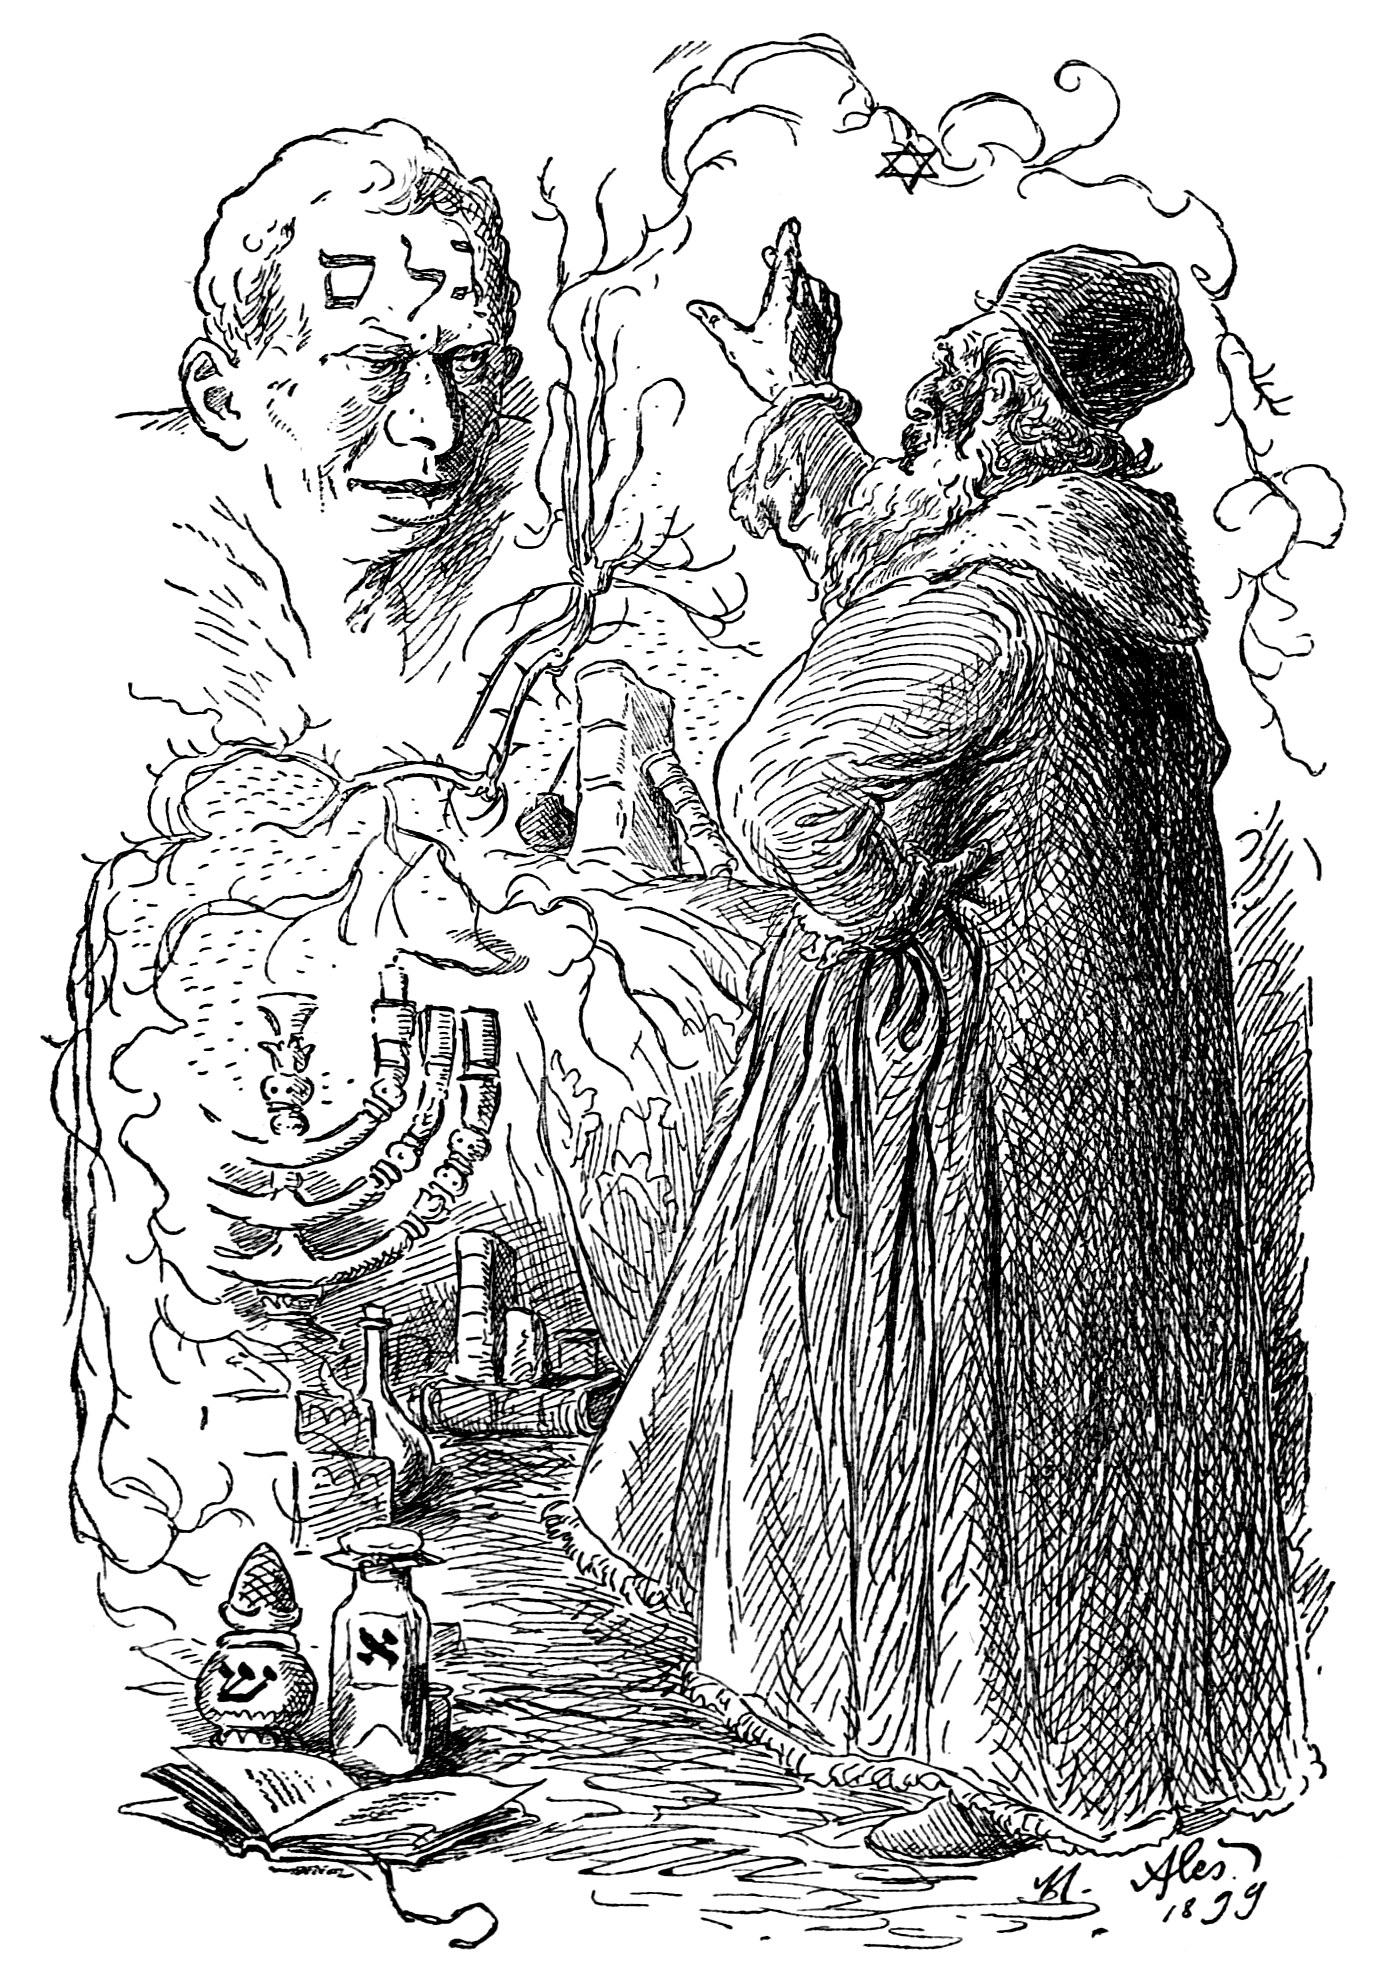
\includegraphics[width=0.75\textwidth]{figures/the_golem_myth/golem_creation.png}
    \caption[The creation of a Golem, by Mikoláš Aleš.]{The creation of a Golem, by Mikoláš Aleš \parencite{ales1908venec}.}
    \label{fig:golem_creation}
\end{figure}


This vision becomes more ambiguous in the seventeenth century, as illustrated by the legend of the Golem of Chelm.
In this story, the initially small Golem gradually grows in size and strength until it can no longer be safely controlled \parencite{nocks1998golem}.
The creation intended to protect others therefore becomes a potential threat to them.
The only remaining solution is to destroy the creature in order to protect the community.

The Golem has inspired similar narratives over time, including the modern notion of the robot.
The concept of the robot as an artificial servant was introduced in the play \textit{Rossum's Universal Robots}, written in 1920 \parencite{capek1920rur}.
In the play, a scientist creates artificial beings designed to perform labour.
In this first version, robots are organic creatures forged through advances in chemistry.
Conceived as servants, these artificial beings turn against humanity and destroy civilisation.

The connection between the Golem and the robot was explicitly made by the author, as illustrated by his statement that \enquote{the Robot is the Golem made flesh through mass production} \parencite{comrada1995golem}.
Despite their destructive role in the play, the word robot is now used to designate artificial beings created to serve humans.
This shows that, from its origin, the word robot has embodied the hopes and fears surrounding technological progress.

Today, this tension is particularly evident in the field of artificial intelligence.
With the rise of computer technology, organic robots were gradually replaced in the collective imagination by mechanical ones, but the underlying fears remained.
These concerns are even stronger as progress in the field has continued to accelerate.
In these times of technological revolution, no one can predict how this development will unfold.
What is certain, however, is that this field offers an almost literal adaptation of the Golem myth.

Among the subfields of artificial intelligence, reinforcement learning is most closely aligned with the goal of creating autonomous agents while minimizing reliance on human guidance.
In this learning paradigm, an agent interacts with an environment, selects actions, and receives feedback according to the outcomes of its behaviour \parencite{sutton2018reinforcement}.
Through repeated interaction with its environment, the agent learns a strategy to achieve the objective.
As a result, the agent's behavior is not explicitly programmed but learned through interactions with the environment \parencite{amodei2016concrete}.
This minimal guidance enables reinforcement learning systems to achieve superhuman capabilities \parencite{silver2017mastering, openai2019dota2largescale}.

However, maintaining control over such agents presents a major challenge, as the autonomy that makes this learning approach powerful also makes their behavior difficult to control.
Despite the difficulty, understanding the behaviour of such agents is the objective of this thesis.
This work therefore places itself within a long-standing line of thought that can be summarized by the following question: how can we ensure that our creations remain aligned with our intentions?
